\section{Attention Models}

  We have seen the power of encoder decoder models, which can be used with a combination of RNNs or CNNs. Since we can plug and play different architectures, we can process and output different types of data.\footnote{CNNs can be used to encode or output images and RNNs can be used to encode or output sequential data.} CNNs were quite strong and have really no problem with scaling ever since the ResNet architecture, but historically, RNNs had two main problems. 
  \begin{enumerate} 
    \item They compute sequentially, since the hidden states must be a function of previous hidden states. This results in a linear time complexity, which is not ideal. 
    \item By encoding the entire sequence in a hidden latent space of dimension $h$, we are essentially trying to compress a possibly very long sequence into a single vector of predetermined dimension. This causes a \textit{bottleneck problem} and words that are further away may be ``forgotten.''
  \end{enumerate}

  We will see that attention solves the second bottleneck problem, and self-attention solves the sequential problem. 

  In general, feed forward networks treat features as independent, convolutional networks focus on relative location and proximity, and RNNs have tend to read in one direction. This may not be the most flexible way to process data, and we have some other problems. 
  \begin{enumerate}
      \item When processing images, we may want our CNN to focus on a specific part of the image. For example, when we see a cat in the corner, other parts of the image does not matter, and we can have our CNN focus on the specific portion of the image containing the cat. 
      \item When reading sentences, different words may be interdependent, even if they are not next to each other, and so we may want to focus on different portions of a sentence (e.g. words 1~3, plus 10~15 which describes an object). 
  \end{enumerate}

  This is where attention comes in to the rescue. Attention is, to some extent, motivated by how we pay visual attention to different regions of an image or correlate words in one sentence. Human attention allows us to focus on certain regions or portions of our data with ``high resolution" while perceiving the surrounding data in ``low resolution." In a nutshell, attention in deep learning can be broadly interpreted as a vector of importance weights. First, we will introduce attention in the general setting, then move onto its specific implementation in RNNs through the seq2seq attention model, and finally its application in CNNs through Vision transformers. 

\subsection{Seq2Seq with Attention}

  The idea of \textbf{attention} provides a solution to this bottleneck problem. Basically, we want to establish connections from the decoder to not just the last hidden state of the encoder, but to all of its nodes. Each encoder node represents some information about each word, and by taking some weighted sum of these nodes, we can choose which one to put this attention on. 

  \begin{definition}[Score Function]
    Before we begin, let's define a metric, called a \textbf{score function}, to determine how similar two words (more specifically, their embeddings) are. The two simplest ways to do this are: 
    \begin{enumerate}
      \item the standard dot product. 
        \begin{equation}
          \mathrm{score}(\mathbf{x}, \mathbf{y}) = \mathbf{x} \cdot \mathbf{y} 
        \end{equation}
      \item cosine similarity. 
        \begin{equation}
          \mathrm{score}(\mathbf{x}, \mathbf{y}) = \frac{\mathbf{x} \cdot \mathbf{y}}{||\mathbf{x}|| \, ||\mathbf{y}||}
        \end{equation}
    \end{enumerate}
  \end{definition}

  Now that we have the score defined, the heart of attention comes with the query, key, value model. The general idea is this: for every prediction we want to make (whether it is classifying something or generating a new output word/token), we want to get its respective query vector and use it to look through key-value dictionary in order to get the most relevant information from it. With this information, combined with the query and whatever other information we have, we can make a prediction. 

  Let's go through this step by step. What we want to do is associate every input hidden node $\mathbf{h}_t$ with a 2-tuple consisting of a key-value pair. 

  \begin{equation}
    \mathbf{h}_t \mapsto (\mathbf{k}_t, \mathbf{v}_t)
  \end{equation}

  and associate every hidden output node $\mathbf{s}_t$ with a query value. 
  \begin{equation}
    \mathbf{s}_T \mapsto \mathbf{q}_t
  \end{equation}

  \begin{definition}[Seq2Seq with Vanilla Attention] 
    Eventually, we would like to learn these key, value, queries, but for now let's focus on the forward propagation. 
    \begin{enumerate}
      \item The input has been sequentially encoded and we have a special start token $\mathbf{s}_0$. 
      \item For $t^\prime = 0$ until the $\mathbf{s}_{T^\prime}$ is the end token, do the following. 
      \begin{enumerate}
        \item Take the query $\mathbf{s}_i$ and compute the attention score $\mathrm{score}(\mathbf{s}_i, \mathbf{h}_t)$ for all $t = 1, \ldots, T$. This determines which encoder hidden state we should pay attention to. 
        \begin{equation}
          \mathbf{e}^{t^\prime} = \big[ \mathrm{score}(\mathbf{s}_{t^\prime}, \mathbf{h}_1 ), \ldots, \mathrm{score}(\mathbf{s}_{t^\prime}, \mathbf{h}_T) \big] \in \mathbb{R}^T
        \end{equation}

        \item We take its softmax to get the \textbf{attention distribution} $\boldsymbol{\alpha}^{t^\prime}$ for this step (a discrete probability distribution) 
        \begin{equation}
          \boldsymbol{\alpha}^{t^\prime} = \mathrm{softmax} (\mathbf{e}^{t^\prime}) \in \mathbb{R}^T
        \end{equation}

        \item We use $\boldsymbol{\alpha}^{t^\prime}$ to take a weighted sum of the encoder hidden states to get the attention output $\mathbf{a}_t$ 
        \begin{equation}
          \mathbf{a}_{t^\prime} = \sum_{t=1}^T \alpha_{t}^{t^\prime} \mathbf{h}_t \in \mathbb{R}^h
        \end{equation}
        which acts as our context vector $\mathbf{C}_{t^\prime}$ that we can now use in our vanilla seq2seq model.\footnote{This weighted sum is a selective summary of the information contained in the values, where the query determines which values to focus on. Attention is a way to obtain a fixed size representation of an arbitrary set of representations (the values), dependent on some other representation (the query).} Note that this context vector is different for every $\mathbf{s}_{t^\prime}$, so at every step we can choose which encoder states/words to focus on. \footnote{This is similar to a hash map where you have a set of key-value pairs. When you have a query, you want to search through the keys to see if it matches the query, and then it returns the value of the matched key. In our case, we have a query, and rather than looking for exact matches, we want to return a similarity score of the query $q_i$ across all $k_i$'s and provide a weighted sum of the corresponding values.} 
      \end{enumerate}
    \end{enumerate}

    Another trick to improve performance is that these attention context vectors can be concatenated with the previous decoder hidden state to get more information in the already decoded part of the sentence.   

    \begin{center}
      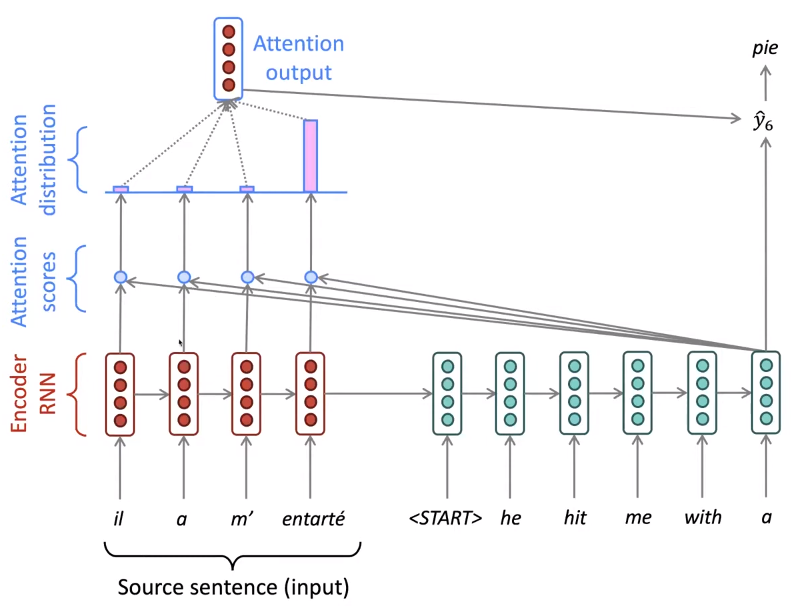
\includegraphics[scale=0.4]{img/seq2seq_attention.png}
    \end{center}
  \end{definition}

  Overall, attention is extremely useful in improving all performance, and it is intuitive with how humans analyze things, too. It significantly improves neural machine translation by allowing the decoder to focus on certain parts of the source. It also provides more ``human-like" model of the machine translation process (you can look back at the source sentence while translating, rather than needing to remember it all). It solves the bottleneck problem and helps with the vanishing gradient problem with these pseudo-residual connections through the context vector. 

  Finally, it provides some interpretability, as we can inspect the attention distribution to see what the decoder was focusing on (which again, we've never set explicitly but was learned by the model). 

  \begin{center}
    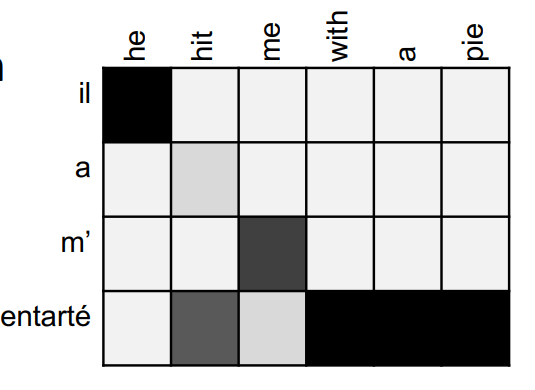
\includegraphics[scale=0.3]{img/attention_distribution.png}
  \end{center}

  \begin{code}
    For an implementation of this in PyTorch, look \href{code/seq2seq_attention.ipynb}{here}.
  \end{code}

  Now let's talk about how these parameters are already learned. The parameters of the model are. 
  \begin{enumerate}
    \item The encoding matrices for the usual seq2seq model: $\mathbf{W}_e, \mathbf{U}_e$. 
    \item Generating key, value, and query vectors for every possible embedding is not practical.\footnote{You would need three $d_{\mathrm{embedding}} \times |\mathcal{V}|$ matrices, where $\mathcal{V}$ is the set of our vocabulary, which can go easily past 500,000 elements.} A more compact way to represent them are through linear maps, so we are learning matrices $\mathbf{Q}, \mathbf{K}, \mathbf{V}$ such that 
    \begin{align*}
      \mathbf{q}_{t^\prime} & = \mathbf{Q} \mathbf{s}_{t^\prime} \\ 
      \mathbf{k}_t & = \mathbf{K} \mathbf{h}_t \\
      \mathbf{v}_t & = \mathbf{V} \mathbf{h}_t
    \end{align*}

    \item We should now have the decoding matrices $\mathbf{W}_d$ that takes in the attention context vector (plus maybe the previous hidden decoder state) and the original matrix $\mathbf{U}_d$. 
  \end{enumerate}
  Therefore, this problem reduces to learning the matrices $\mathbf{W}_e, \mathbf{U}_e, \mathbf{Q}, \mathbf{K}, \mathbf{V}, \mathbf{W}_d, \mathbf{U}_d$. 

  \begin{example}[Score Functions]
    Having additional flexibility with the score functions can also improve learning. We provide more examples here, which give more parameters to learn as well.  
    \begin{enumerate}
      \item The general attention model allows us to train a shared-weight matrix, allowing for $s \neq h$. 
      \[e^{t^\prime}_t = \mathrm{score}(\mathbf{s}_{t^\prime}, \mathbf{h}_t) = \mathbf{s}_{t^\prime}^T \mathbf{W}_a \mathbf{h}_t \in \mathbb{R}\]
      However, it may seem like there are too many parameters in $\mathbf{W}_a$, having to learn $sh$ values. 

      \item The reduced rank multiplicative attention uses low rank matrices, allowing us to learn only $ks + kh$ parameters for matrices $\mathbf{U}_a \in \mathbb{R}^{k \times s}, \mathbf{V}_a \in \mathbb{R}^{k \times h}$ where $k << s, h$. 
      \[e^{t^\prime}_t = \mathrm{score}(\mathbf{s}_{t^\prime}, \mathbf{h}_t) = \mathbf{s}_{t^\prime}^T (\mathbf{U}_a^T \mathbf{V}_a) \mathbf{h}_t = (\mathbf{U}_a \mathbf{s}_{t^\prime})^T (\mathbf{V}_a \mathbf{h}_t) \in \mathbb{R}\]

      \item Additive attention uses a neural net layer defined 
      \[e^{t^\prime}_t = \mathbf{v}_a^T \mathrm{tanh}(\mathbf{W}_a \mathbf{h}_t + \mathbf{V}_a \mathbf{s}_{t^\prime}) \in \mathbb{R}\]
      where $\mathbf{W}_a \in \mathbb{R}^{r \times h}, \mathbf{V}_a \in \mathbb{R}^{r \times s}$ are weight matrices, $\mathbf{v}_a \in \mathbb{R}^r$ is a weight vector, and $r$ (the attention dimensionality) is a hyperparameter. 
    \end{enumerate}
  \end{example}

  This can be naturally extended to other architectures, as we will explore later. 

  \begin{example}[Images]
    Given an image of size $224 \times 224$, we can make patches of size $16 \times 16$, and then flatten them to get a $196 \times 768$ matrix with a 2-dimensional positional encoding scheme. We can then apply a linear transformation to get the query, key, and value vectors.
  \end{example}

